\documentclass{standalone}

\usepackage[utf8]{inputenc}
\usepackage[T1]{fontenc}
\usepackage{fontawesome}
\usepackage{tikz}
\usetikzlibrary{arrows}
\begin{document}

\begin{tikzpicture}
\node at (9.5,18) {\Huge \textbf{Erdgeschoss}};
%\draw (0,0) -- (20,0) -- (20,20) -- (0,20) -- (0,0); % Canvas
% \draw (,) -- (,);
\fill[red!60] (4,8) rectangle (15,16);
\fill[yellow!20] (1,1) -- (1,19) -- (3,19) -- (3,4.5) -- (4,4.5) -- (4,8) -- (15,8) -- (15,5) -- (18,5) -- (18,3) -- (16,3) -- (16,0) -- (15,0) -- (15,1) -- (15,1) -- (4,1) -- (4,0) -- (3,0) -- (3,1) -- (1,1);
\fill[gray!30] (16,0) rectangle (18,3);
\fill[gray!30] (16,5) rectangle (18,19);

\draw (1,1) -- (1,17);
\draw (3,4) -- (3,17);
\draw (4,4.5) -- (4,16);
\draw (3,4.5) -- (4,4.5);
\draw (4,16) -- (15,16);
\draw (11,8) -- (11,16);
\draw (15,0) -- (15,2);
\draw (15,5) -- (15,16);
\draw (16,0) -- (16,3.5);
\draw (16,4.5) -- (16,17);
\draw (18,0) -- (18,3.5);
\draw (18,4.5) -- (18,17);
\draw (14,3) -- (18,3);
\draw (15,0) -- (18,0);
\draw (1,1) -- (1.5,1);
\draw (2.5,1) -- (3,1);
\draw (1,3) -- (1.5,3);
\draw (2.5,3) -- (4,3);
\draw (3,0) -- (3,2);
\draw (4,0) -- (4,3);
\draw (3,0) -- (4,0);
\draw (4,1) -- (5,1);
\draw (6,1) -- (13,1);
\draw (14,1) -- (15,1);
\draw (12,1) -- (12,3);
\draw (12,3) -- (13,3);
\draw (15,5) -- (18,5);
\draw (5,8) -- (10,8);
\draw (12,8) -- (14,8);
\draw (6,7) -- (9,7) -- (9,8);

\node at (7.5,14) {\Huge \textbf{Hörsaal 1}};
\node at (7.5,12) {\LARGE \textbf{Plenum}};
\node at (13,14) {\Huge \textbf{Hörsaal 2}};

\draw[dashed] (1,17) -- (1,19);
\draw[dashed] (3,17) -- (3,19);
\draw[dashed] (16,17) -- (16,19);
\draw[dashed] (18,17) -- (18,19);
\draw[->, line width=1mm] (2,17.5) -- (2,18.5);
\node[rotate=-90] at (2,12) {\LARGE \textbf{ewiges Frühstück, Orgabüro im PI}};
%\draw[->, line width=1mm] (19,12) -- (19,13);
%\node[rotate=-90] at (19,9) {\LARGE \textbf{ewiges Frühstück}};
\node at (7.5,7.5) {\huge \faMale};
\node at (8,7.5) {\huge \faFemale};
%down stairs
\draw (6,7.8) -- (6.2,7.8);
\draw (6.2,7.6) -- (6.4,7.6);
\draw (6.4,7.4) -- (6.6,7.4);
\draw (6.6,7.2) -- (6.8,7.2);
\draw (6.2,7.8) -- (6.2,7.6);
\draw (6.4,7.6) -- (6.4,7.4);
\draw (6.6,7.4) -- (6.6,7.2);
\draw[->, line width=0.3mm] (6.6,7.8) -- (7,7.4);

\draw (3.2,1) -- (3.4,1);
\draw (3.4,1.2) -- (3.6,1.2);
\draw (3.6,1.4) -- (3.8,1.4);
\draw (3.2,0.8) -- (3.2,1);
\draw (3.4,1) -- (3.4,1.2);
\draw (3.6,1.2) -- (3.6,1.4);
\draw[->, line width=0.3mm] (3.2,1.4) -- (3.6,1.8);

\draw (15.2,1) -- (15.4,1);
\draw (15.4,1.2) -- (15.6,1.2);
\draw (15.6,1.4) -- (15.8,1.4);
\draw (15.2,0.8) -- (15.2,1);
\draw (15.4,1) -- (15.4,1.2);
\draw (15.6,1.2) -- (15.6,1.4);
\draw[->, line width=0.3mm] (15.2,1.4) -- (15.6,1.8);
\node[rotate=-90] at (19,9) {\LARGE \textbf{}};%Platzhalter
\end{tikzpicture}

\end{document}
